\begin{figure}[h]
    \centering
    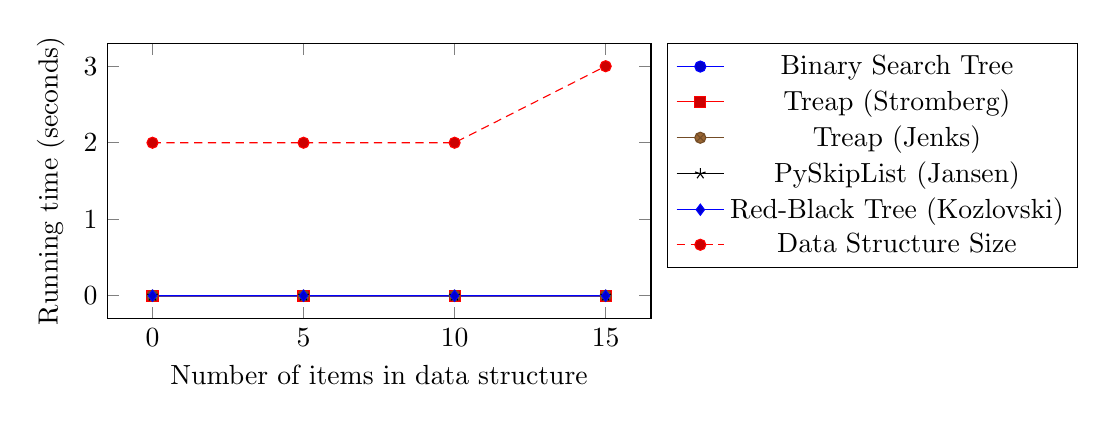
\begin{tikzpicture}
        \begin{axis}[
            xlabel={Number of items in data structure},
            ylabel={Running time (seconds)},
            title={},
            width=0.7\textwidth,
            height=2in,
            legend pos=outer north east
        ]
		\addplot coordinates {
			(0, 3.4133204831855606e-06)
			(5, 3.212536925351235e-06)
			(10, 2.3090109150961913e-06)
			(15, 2.8109698096822947e-06)
		};
		\addplot coordinates {
			(0, 6.9270327452885735e-06)
			(5, 7.529383418791551e-06)
			(10, 3.312928704268398e-06)
			(15, 3.814887598854501e-06)
		};
		\addplot coordinates {
			(0, 6.224290292867855e-06)
			(5, 7.228208082040062e-06)
			(10, 3.6141040410201755e-06)
			(15, 2.30901091509648e-06)
		};
		\addplot coordinates {
			(0, 1.1545054575480667e-05)
			(5, 1.1143487459812015e-05)
			(10, 5.722331398281752e-06)
			(15, 1.0942703901977111e-05)
		};
		\addplot coordinates {
			(0, 8.031342313377654e-06)
			(5, 1.1143487459812015e-05)
			(10, 7.629775197709002e-06)
			(15, 2.8109698096822947e-06)
		};
		\addplot coordinates {
			(0, 2)
			(5, 2)
			(10, 2)
			(15, 3)
		};
        \legend{Binary Search Tree, Treap (Stromberg), Treap (Jenks), PySkipList (Jansen), Red-Black Tree (Kozlovski), Data Structure Size}
        \end{axis}
    \end{tikzpicture}
    \caption{Average of 3 operations, benchmarked every 5, starting at 0.}
\end{figure}